\documentclass[nooutcomes]{ximera}
%\documentclass[space,handout,nooutcomes]{ximera}

% For preamble materials

\usepackage{pgf,tikz}
\usepackage{mathrsfs}
\usetikzlibrary{arrows}
\usepackage{framed}
\usepackage{amsmath}
\pgfplotsset{compat=1.17}

\def\fixnote#1{\begin{framed}{\textcolor{red}{Fix note: #1}}\end{framed}}  % Allows insertion of red notes about needed edits
%\def\fixnote#1{}

\def\detail#1{{\textcolor{blue}{Detail: #1}}}   

\pdfOnly{\renewenvironment{image}[1][]{\begin{center}}{\end{center}}}

\graphicspath{
  {./}
  {chapter1/}
  {chapter2/}
  {chapter4/}
  {proofs/}
  {graphics/}
  {../graphics/}
}

\newenvironment{sectionOutcomes}{}{}


%%% This set of code is all of our user defined commands
\newcommand{\bysame}{\mbox{\rule{3em}{.4pt}}\,}
\newcommand{\N}{\mathbb N}
\newcommand{\C}{\mathbb C}
\newcommand{\W}{\mathbb W}
\newcommand{\Z}{\mathbb Z}
\newcommand{\Q}{\mathbb Q}
\newcommand{\R}{\mathbb R}
\newcommand{\A}{\mathbb A}
\newcommand{\D}{\mathcal D}
\newcommand{\F}{\mathcal F}
\newcommand{\ph}{\varphi}
\newcommand{\ep}{\varepsilon}
\newcommand{\aph}{\alpha}
\newcommand{\QM}{\begin{center}{\huge\textbf{?}}\end{center}}

\renewcommand{\le}{\leqslant}
\renewcommand{\ge}{\geqslant}
\renewcommand{\a}{\wedge}
\renewcommand{\v}{\vee}
\renewcommand{\l}{\ell}
\newcommand{\mat}{\mathsf}
\renewcommand{\vec}{\mathbf}
\renewcommand{\subset}{\subseteq}
\renewcommand{\supset}{\supseteq}
%\renewcommand{\emptyset}{\varnothing}
%\newcommand{\xto}{\xrightarrow}
%\renewcommand{\qedsymbol}{$\blacksquare$}
%\newcommand{\bibname}{References and Further Reading}
%\renewcommand{\bar}{\protect\overline}
%\renewcommand{\hat}{\protect\widehat}
%\renewcommand{\tilde}{\widetilde}
%\newcommand{\tri}{\triangle}
%\newcommand{\minipad}{\vspace{1ex}}
%\newcommand{\leftexp}[2]{{\vphantom{#2}}^{#1}{#2}}

%% More user defined commands
\renewcommand{\epsilon}{\varepsilon}
\renewcommand{\theta}{\vartheta} %% only for kmath
\renewcommand{\l}{\ell}
\renewcommand{\d}{\, d}
\newcommand{\ddx}{\frac{d}{dx}}
\newcommand{\dydx}{\frac{dy}{dx}}


\usepackage{bigstrut}


\title{Proof by Picture 1}
\author{Bart Snapp and Brad Findell}
\begin{document}
\begin{abstract}
Short-answer proofs by pictures. 
\end{abstract}
\maketitle


\begin{problem}
Explain how the following picture ``proves'' that
  the area of a right triangle is half the base times the height.
\begin{image}
\definecolor{qqwuqq}{rgb}{0.,0.392,0.}
\begin{tikzpicture}[line cap=round,line join=round,>=triangle 45,x=1.0cm,y=1.0cm]
%\clip(-4.1,-0.1) rectangle (8.1,3.1);
\draw[line width=0.8pt,color=qqwuqq,fill=qqwuqq,fill opacity=0.10] (0.28,0.) -- (0.28,0.28) -- (0.,0.28) -- (0.,0.) -- cycle; 
\draw [line width=0.8pt] (0.,3.)-- (0.,0.);
\draw [line width=0.8pt] (0.,0.)-- (4.,0.);
\draw [line width=0.8pt] (4.,0.)-- (0.,3.);
\draw [line width=0.8pt,dash pattern=on 2pt off 2pt] (0.,3.)-- (4.,3.);
\draw [line width=0.8pt,dash pattern=on 2pt off 2pt] (4.,3.)-- (4.,0.);
\draw [color=gray] (-4.,0.) circle (0.2pt);
\draw [color=gray] (8.,0.) circle (0.2pt);
%\draw[color=black] (0.54,-0.15) node {$f$};
\end{tikzpicture}
%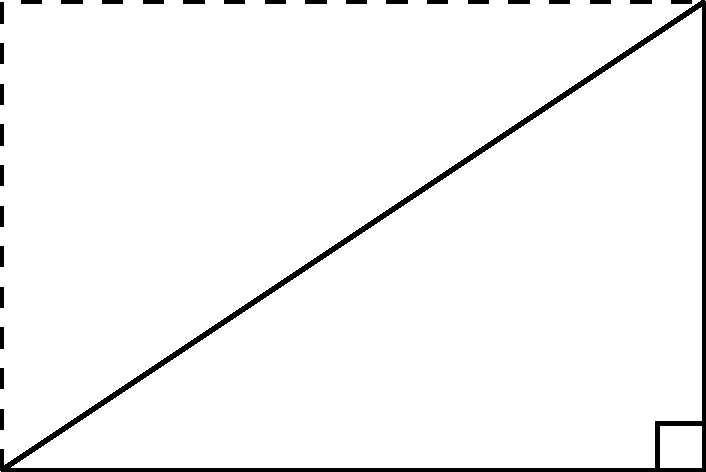
\includegraphics{pbpAreaRight.png}
\end{image}
\begin{freeResponse}
\begin{hint}
The area of the rectangle is base times height.  The rectangle is made up of two congruent right triangles.  Because congruent triangles have the same area, the area of each right triangle is \wordChoice{\choice{equal to}\choice[correct]{half}\choice{double}} the area of the rectangle.  
\end{hint}
\end{freeResponse}
\end{problem}

\begin{problem}
Suppose you know that the area of a \textbf{right} triangle is
  half the base times the height. Explain how the following picture
  ``proves'' that the area of \textbf{every} triangle is half the base times the
  height.
\begin{image}
\definecolor{qqwuqq}{rgb}{0.,0.392,0.}
\begin{tikzpicture}[line cap=round,line join=round,>=triangle 45,x=1.0cm,y=1.0cm]
%\clip(-0.5,-0.05) rectangle (5,2.55);
\draw[line width=0.8pt,color=qqwuqq,fill=qqwuqq,fill opacity=0.1] (3.,0.1954) -- (2.8046,0.1954) -- (2.8046,0.) -- (3.,0.) -- cycle; 
\draw[line width=0.8pt,color=qqwuqq,fill=qqwuqq,fill opacity=0.1] (3.1954,0.) -- (3.1954,0.1954) -- (3.,0.1954) -- (3.,0.) -- cycle; 
\draw [line width=0.8pt] (0.,0.)-- (3.,2.5);
\draw [line width=0.8pt] (3.,2.5)-- (4.,0.);
\draw [line width=0.8pt] (4.,0.)-- (0.,0.);
\draw [line width=0.8pt] (0.,0.)-- (3.,0.);
\draw [line width=0.8pt] (3.,0.)-- (4.,0.);
\draw [line width=0.8pt,dash pattern=on 2pt off 2pt] (3.,0.)-- (3.,2.5);
\draw [color=gray] (-4.,0.) circle (0.1pt);
\draw [color=gray] (8.,0.) circle (0.1pt);
\end{tikzpicture}
%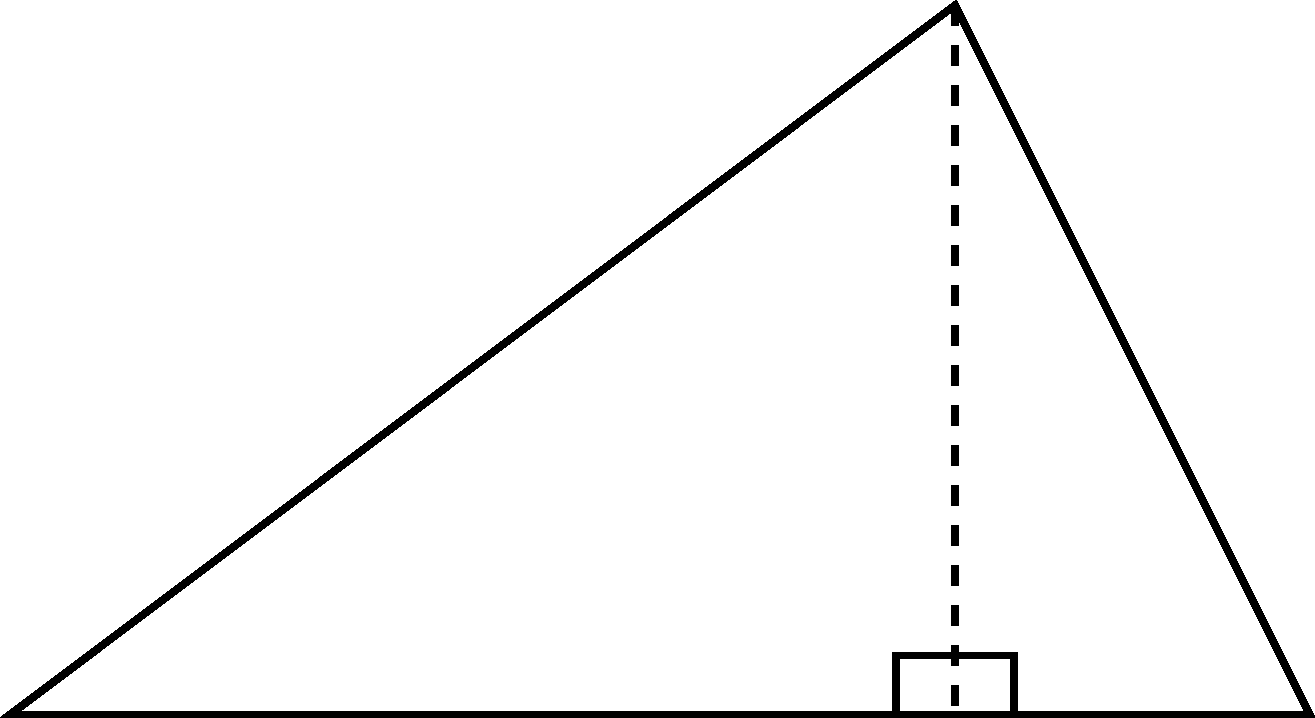
\includegraphics{pbpDisTri.png}
\end{image}

\begin{freeResponse}
\begin{hint}
The whole triangle is made up of two right triangles.  Call the bases of the small right triangles $b_1$ and $b_2$, and call the base of the large (combined) triangle $b$.  Then $b=b_1+b_2$, and the three triangles all have the same height, $h$.   The area of the whole triangle is the sum of the areas of the two right triangles:  
\[
\mathrm{area} =  \frac{hb_1}{2}+ \frac{hb_2}{2}= \frac{h(b_1 + b_2)}{2} = \answer{bh/2}
\]
because $b=b_1+b_2$.
\end{hint}
\end{freeResponse}
\end{problem}

\begin{problem}
Now suppose that a student, say \textit{Geometry Giorgio} attempts to
solve a similar problem. Again knowing that the area of a right
triangle is half the base times the height, he draws the following
picture:
\begin{image}
\begin{tikzpicture}[line cap=round,line join=round,>=triangle 45,x=1.0cm,y=1.0cm]
%\clip(-0.5,-0.05) rectangle (5.25,2.55);
\draw [line width=0.8pt,dash pattern=on 2pt off 2pt] (0.,0.)-- (0.,2.5);
\draw [line width=0.8pt,dash pattern=on 2pt off 2pt] (0.,2.5)-- (5.,2.5);
\draw [line width=0.8pt,dash pattern=on 2pt off 2pt] (5.,2.5)-- (5.,0.);
\draw [line width=0.8pt] (5.,2.5)-- (2.,0.);
\draw [line width=0.8pt] (5.,2.5)-- (0.,0.);
\draw [line width=0.8pt] (0.,0.)-- (2.,0.);
\draw [line width=0.8pt,dash pattern=on 2pt off 2pt] (2.,0.)-- (5.,0.);
\draw [color=white] (-4.,0.) circle (0.2pt);
\draw [color=white] (8.,0.) circle (0.2pt);
\end{tikzpicture}
%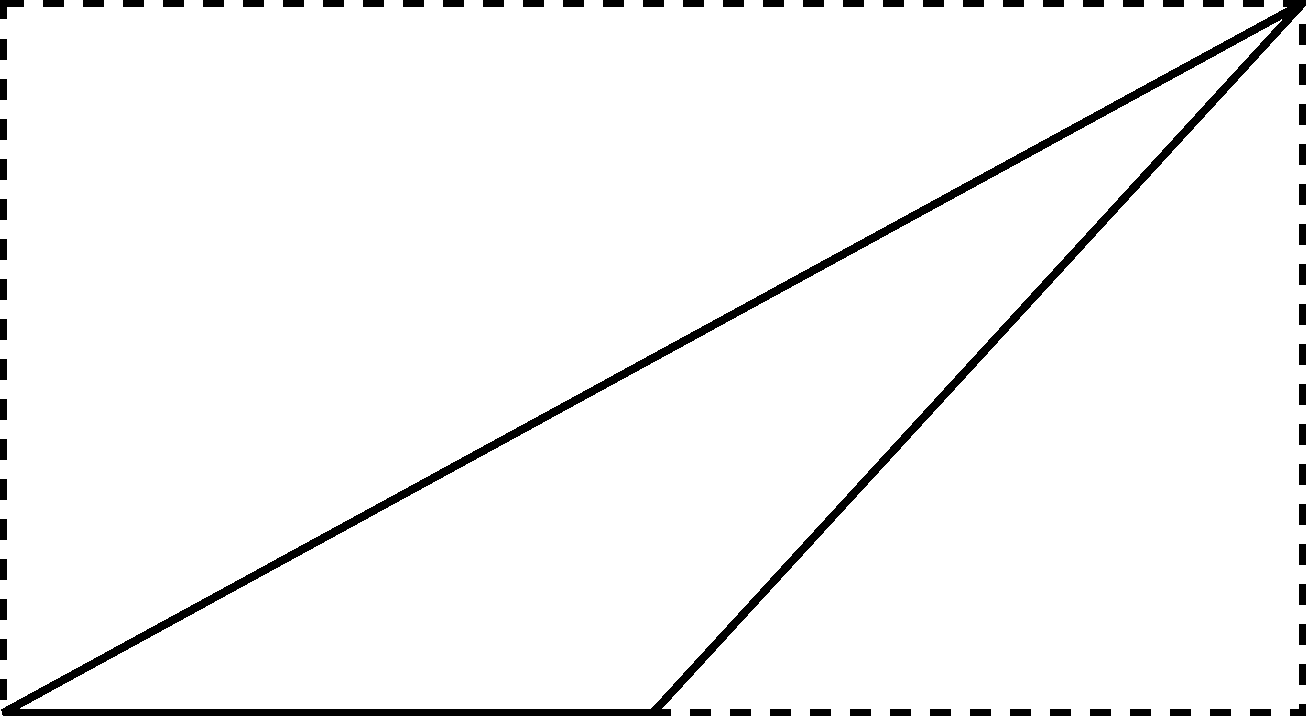
\includegraphics{pbpDisTriGio.png}
\end{image}
\textit{Geometry Giorgio} states that the diagonal line cuts the
rectangle in half, and thus the area of the triangle is half the base
times the height. Is this correct reasoning? If so, give a complete
explanation. If not, give correct reasoning based on \textit{Geometry
  Giorgio's} picture.
\begin{freeResponse}
\begin{hint}
The triangle is not half the rectangle.  Furthermore, the rectangle does not have the same base as the triangle, so ``base times height'' is unclear.  The following picture allows us to distinguish these bases:  
\begin{image}
\begin{tikzpicture}[line cap=round,line join=round,>=triangle 45,x=1.0cm,y=1.0cm]
%\clip(-0.5,-0.05) rectangle (5.25,2.65);
\draw [line width=0.8pt,dash pattern=on 2pt off 2pt] (0.,0.)-- (0.,2.5);
\draw [line width=0.8pt,dash pattern=on 2pt off 2pt] (0.,2.5)-- (5.,2.5);
\draw [line width=0.8pt,dash pattern=on 2pt off 2pt] (5.,2.5)-- (5.,0.);
\draw [line width=0.8pt] (5.,2.5)-- (2.,0.);
\draw [line width=0.8pt] (5.,2.5)-- (0.,0.);
\draw [line width=0.8pt] (0.,0.)-- (2.,0.);
\draw [line width=0.8pt,dash pattern=on 2pt off 2pt] (2.,0.)-- (5.,0.);
\draw[color=black] (1.1,-0.2) node {$b$};
\draw[color=black] (3.5,-0.2) node {$x$};
\draw[color=black] (5.2,1.3) node {$h$};
\draw [color=gray] (-4.,0.) circle (0.2pt);
\draw [color=gray] (8.,0.) circle (0.2pt);
\end{tikzpicture}
%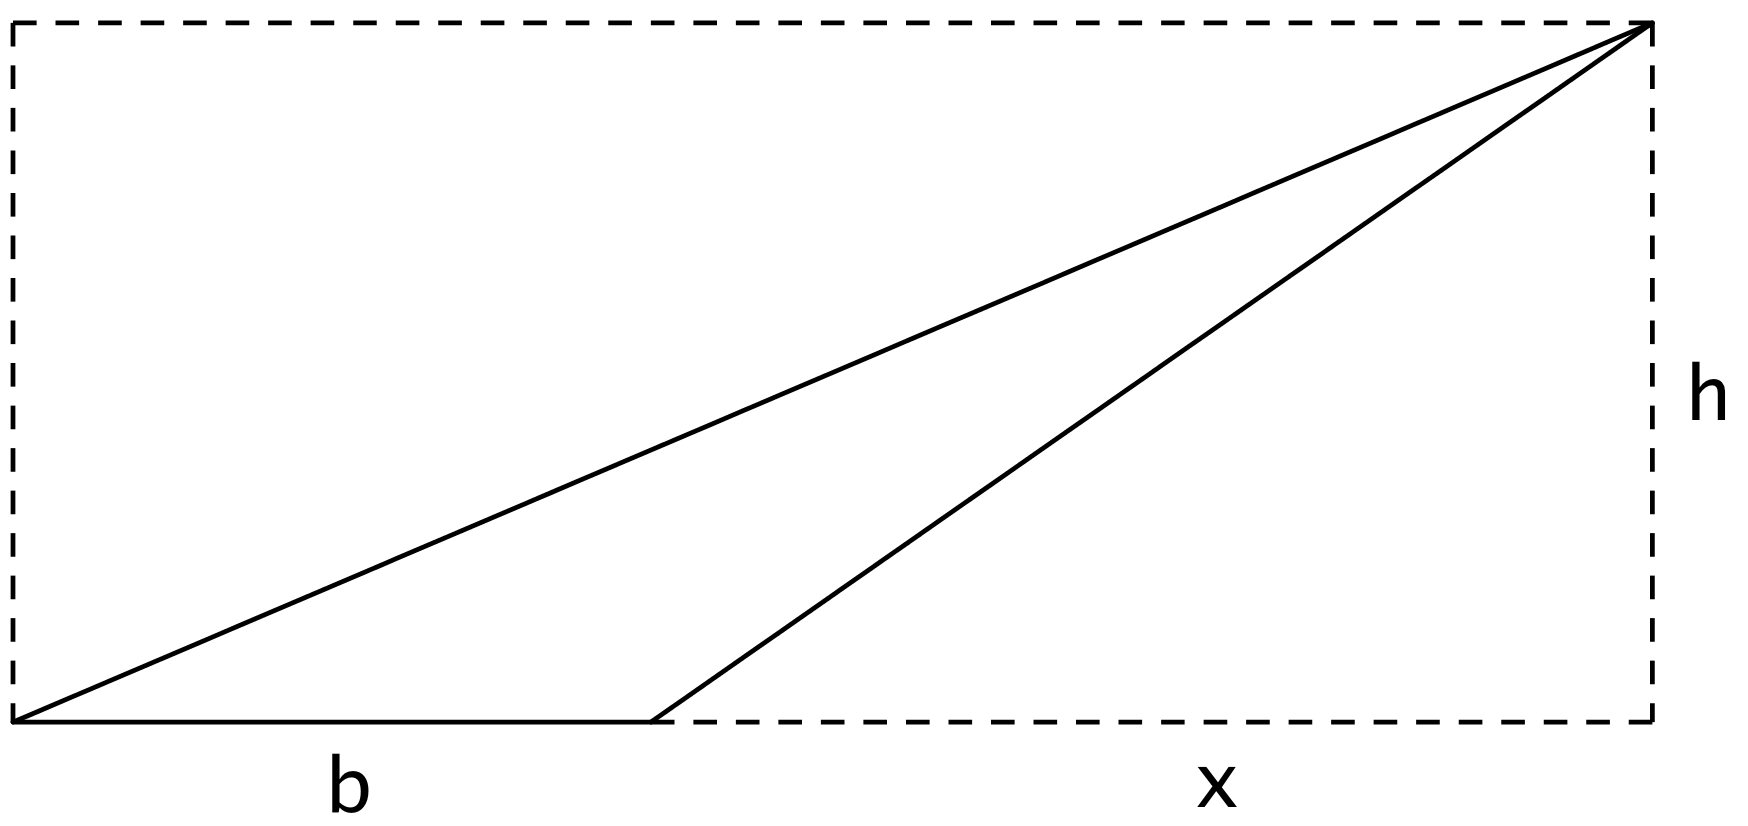
\includegraphics{triangleArea.png}
\end{image}
One way to compute the area of the solid triangle is to (1) compute the area right triangle that is the lower half of the rectangle (with base $b+x$) and then (2) subtract the area of the small right triangle (with base $x$): 
\[
\mathrm{area} =  \answer{\frac{h(b+x)}{2}} - \answer{\frac{hx}{2}}= \frac{hb}{2} + \frac{hx}{2} - \frac{hx}{2} = \answer{\frac{hb}{2}}
\]
\end{hint}
\end{freeResponse}
\end{problem}


\end{document}
